\subsection{Reinforcement learning}

We present a Reinforcement learning (RL) based framework to explore and optimize the mapping of instructions to SE in an unsupervised manner, guided by a reward function that informs the mapping algorithm about the quality of the mapping at each step. 

\subsection{Overview}
Proximal Policy Optimization (PPO) is an RL method widely used for continuous and discrete action problems. It trains actor and critic models (represented as a neural networks). 
The actor model outputs actions (node placements) given an observation of the current state of the SE. The critic model is trained to predict the expected reward given an action in the current state. 
Our SE mapping task is formulated as a discrete action problem where samples of SE state, actions performed, and rewards obtained at each time step are collected after executing the actions provided by the actor model in simulation. These samples are stored in a buffer that is used as data to train the models. 
The key components of our RL method are as follows:
\begin{itemize}
  \item States: In our case, the state is represented by a concatenation of an array of features of placed nodes, a selected node to be placed next and an embedding of the whole computation graph. 
  \item Action: The action at each step is a tuple \((N,T,I)\) where $N$ is the node to be placed and $T$ and $I$ are the tile and initiation interval at which the node $N$ is to be placed.
  \item Reward function: The reward obtained is based on the number of cycles tak-en to execute all nodes.
  \item Transition function: The transition function gives the probability distribution over next states given the current state and the action to be performed.
\end{itemize}


 The actor model is trained to produce actions from sample states obtained during simulation and the critic model is trained to match the sampled rewards from the actions produced by the actor using a surrogate loss function. This sample and train process is repeated over various iterations. In this manner, the problem search space is explored using the reward function as a heuristic.
Figure \ref{fig:ppo} shows the overall RL framework. 
\textcolor{red}{After node placements, routing info and configurations for programming each tile are saved for final output.}

\begin{figure}[h]
  \centering
  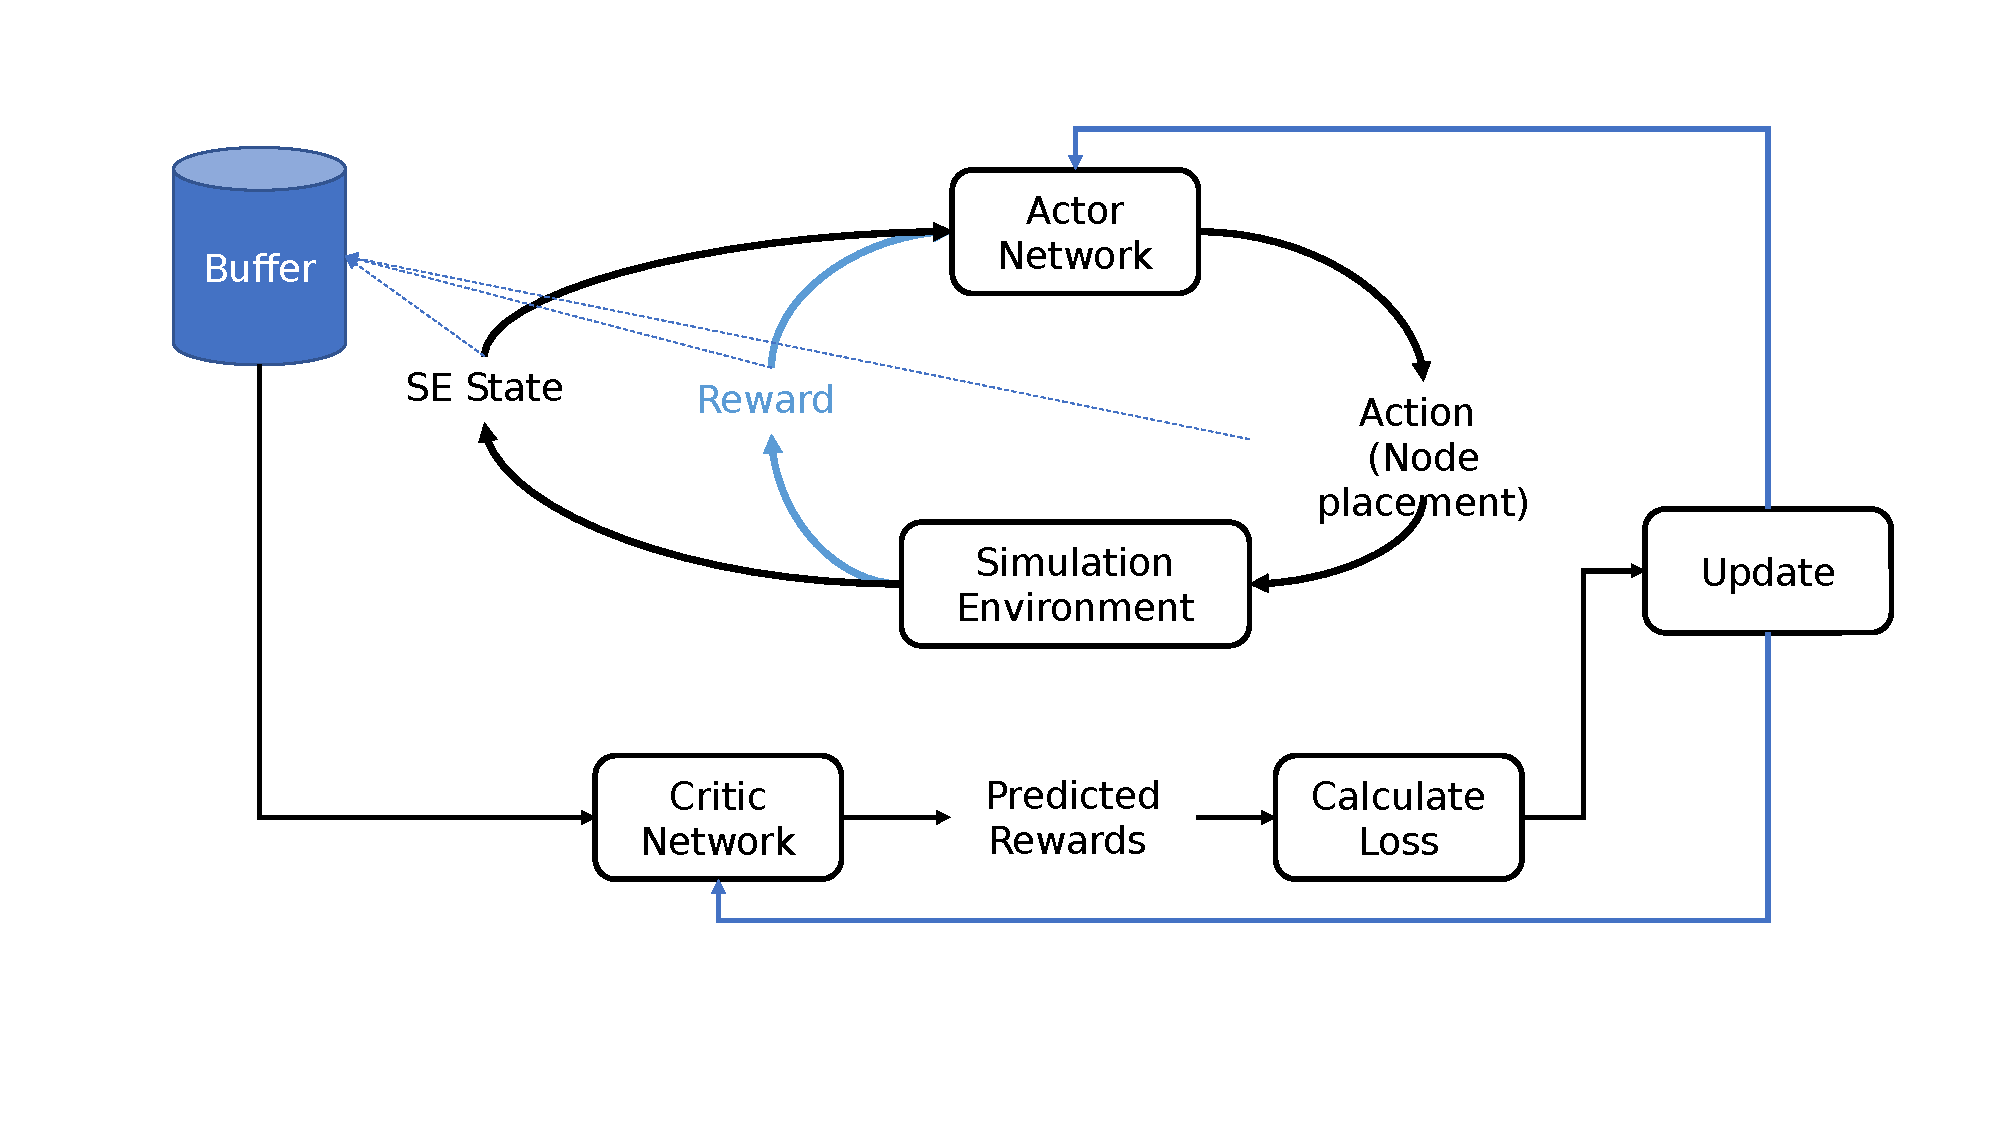
\includegraphics[width=\linewidth]{fig/ppo.pdf}
  \caption{Diagram of the RL framework showing the role of actor and critic networks during RL training. }
  \label{fig:ppo}
\end{figure}

\subsection{Environment Design}

\subsection{Model design}

The actor and critic models architecture is shown in figure \ref{fig:model}. 
The input is separated in two categories: static and dynamic data. 
Static data is information that doesn't change as nodes are being placed, such as: computation graph and tile memory constraint.
Device state, node to be placed and placed node latencies are dynamic data that changes during placement.

Tile memory variables need to be placed in a tile so that operation can use that variable. 
This memory constraint is captured as memory dependency array. 
Tile memory constraints are incorporated into nodes in the computation graph. 
The computation graph has each node representing an instruction. 
The node features are tile memory dependencies. 
A Graph Neural Network (GNN) is used to process node dependencies and create an embedding for each node. 
An attention module is applied to the embedding matrix to select which dependency nodes are relevant to the current node to be placed. The dynamic data is fed into a MLP model to 
create another embedding to represent current state. 
The two embeddings are combined and fed into another MLP model to 
create actions. 
Invalid actions are masked before being sent to the reward function. Masking was shown to be effective in RL setting \cite{Shengyi_mask}.

\begin{figure}[h]
  \centering
  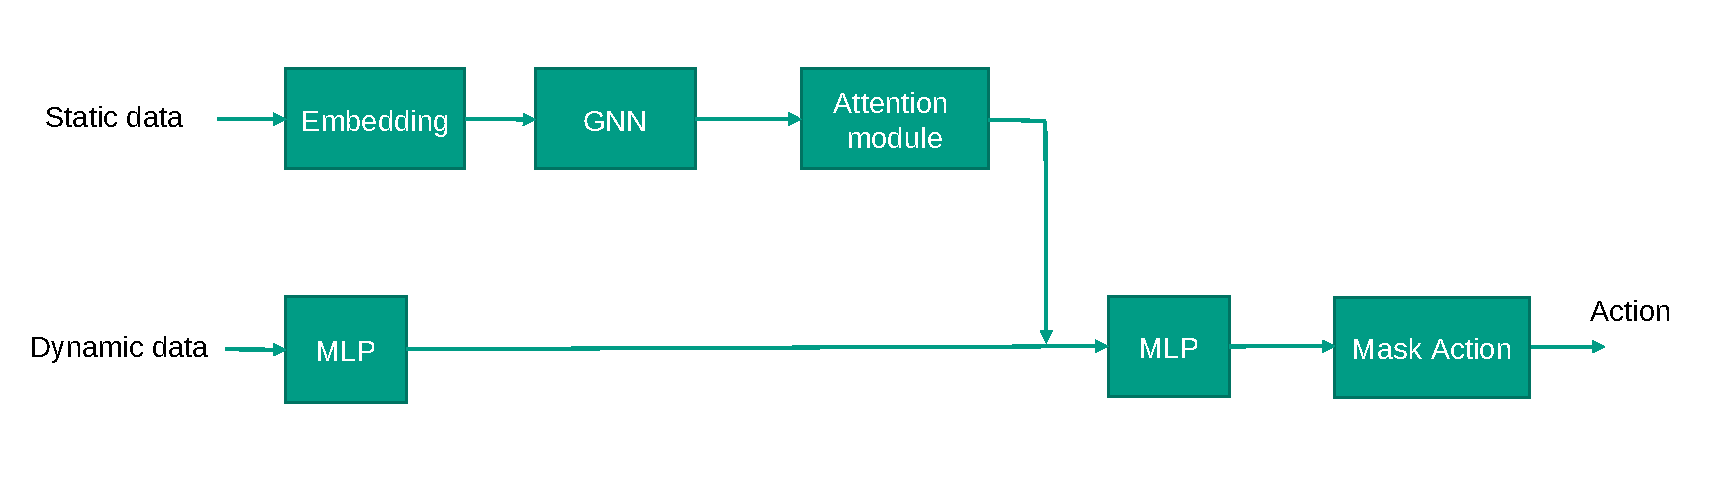
\includegraphics[width=\linewidth]{fig/model.pdf}
  \caption{Actor and critic model architecture. GNN is used to process the computation graph (static data). 
  Attention module gives importance to relevant nodes. The embedding created from dynamic data is combined with static data embedding. 
  A final MLP model is used to generate actions. Actions are masked to ensure only valid actions are produced. }
  \label{fig:model}
\end{figure}

